\chapter{实验}


在本章中对k-means问题使用本文的核心集框架,并在真实数据集上进行实验。

\section{实验设置}
\textbf{k-means/(k-median) 聚类(有离群点):}目标是找到 \( k \) 个聚类中心 \(\text{Cen} = \{c_1, c_2, \cdots, c_k\} \subset \mathbb{R}^d\);k-means(k-medians)聚类的成本函数(或k-means聚类的成本函数)对于每个 \( x \in \mathbb{R}^d \) 是
\[
f(\text{Cen}, x) = \min_{c_i \in \text{Cen}} d(c_i, x)^2 \quad (\text{或 } d(c_i, x))
\]
其中 \( d(c_i, x) \) 表示 \( c_i \) 和 \( x \) 之间的欧几里得距离。


所有算法均在一台配备Intel Xeon E5-2680 v4 CPU(2.40GHz,56核)和250GB内存的服务器上使用Python实现。

\textbf{算法:}我们使用三种基于采样的核心集算法,均匀采样,分层采样以及重要性采样作为框架中的黑盒算法$\mathcal{A}$,并与不使用框架下的这些算法对比。
图示中带有后缀“+”的算法表示使用了本文的框架。基础采样方法分别记为“Uniform”,“GSP”,“Importance”,而使用框架的方法分别记为“Uniform+”,“Stratified+”,“Importance+”。对于许多包含离群点的优化问题,一种常用的策略是交替最小化(例如\cite{DBLP:conf/sdm/ChawlaG13})。
在每次迭代中,首先检测出损失最大的z个异常值,然后在剩下的n-z个点上运行现有算法(不考虑离群点);
然后基于获得的新解更新z个异常值。
该算法重复这一策略,直到解稳定为止。
对于带有异常值的k-means聚类,我们使用“k-means++”方法来选取初始中心,
然后运行k-means--算法\cite{DBLP:conf/sdm/ChawlaG13}。
我们将这些算法应用于获得的核心集上。

\textbf{数据集:}
我们在四个数据集上进行实验:MNIST,CIFAR-10,Covertype和USCensus。对于每个数据集合,我们额外生成一定比例的$\mathcal{N}(0,200)$作为额外噪声。
\textbf{MNIST} 数据集包含70000个手写数字图像,每个图像有784个像素特征,用于分类任务。我们将数据集中的前60000个样本用作训练数据。
\textbf{CIFAR-10} 数据集包含60000张32x32彩色图像,这些图像分为10个类别,每个类别有6000张图像。我们将数据集中的前50000张图像用作训练数据。
\textbf{Covertype} 数据集包含581012个实例,每个实例有54个地理特征,用于预测森林覆盖类型。数据集中有7种覆盖类型。
\textbf{USCensus} 数据集包含1990年美国人口普查数据,包含2458285个实例和68个特征。为了生成异常值用于无监督学习任务k-means聚类,USCensus数据集没有给出种类数,本实验中选择种类数为10。

\section{实验结果分析}

在常规的无监督学习任务中,核心集往往通过计算各种定义的损失偏差和时间加速比评估其性能。
在本实验中,我们使用两种损失偏差,即考虑离群点和不考虑离群点的损失偏差,分别计为$\mathbf{LR}_z$和
$\mathbf{LR}$,下标z表示核心集构建过程(以及kmeans算法)中选择的离群点的数量(权重合)。
\begin{equation*}
    \mathbf{LR} = \max\left\{\frac{f(\theta^*_C,C)}{f(\theta^*_X,X)},\frac{f(\theta^*_X,X)}{f(\theta^*_C,C)}\right\},\quad
    \mathbf{LR}_z = \max\left\{\frac{f_z(\theta^*_C,C)}{f_z(\theta^*_X,X)},\frac{f_z(\theta^*_X,X)}{f_z(\theta^*_C,C)}\right\}
\end{equation*}
其中$\theta^*_{X(C)}$是算法在$X(C)$上使用k-means算法得到的解,核心集大小和加速比分别记为$|C|$和$\mathbf{SR}$。
本实验中有一对重要参数(noise\_ratio,outliers\_ratio)。noise\_ratio表示我们在数据集中额外生成噪声的比例,
outlier\_ratio表示我们在构建核心集和运行kmeans算法时使用的参数,和分析中的离群点数量z直接相关。我们发现,对于不同的参数对,
评价指标$\mathbf{LR}_z$相较$\mathbf{LR}$而言有较大的波动,这说明该评价指标一定程度衡量了鲁棒性,也意味着我们需要针对数据集和算法选择更合适的参数。
表\ref{tab:mnist_combined}展示了在MNIST数据集上不同参数的的实验结果。更多的实验图表详见附录。


\begin{table}[h!]
  \centering
  \caption{(0.2,0.05) 和 (0.05,0.2) - MNIST数据集效果}
  \begin{tabular}{|c|c|c|c|c|c|}
  \hline
  \textbf{方法} & $|C|$ & \textbf{(0.05,0.2) $\mathbf{LR}$} & \textbf{(0.2,0.05) $\mathbf{LR}$} & \textbf{(0.05,0.2) $\mathbf{LR}_z$} & \textbf{(0.2,0.05) $\mathbf{LR}_z$} \\
  \hline
  \multirow{3}{*}{\textbf{Uniform}} 
    & $3 \times 10^3$  & 1.0202 & 1.0277 & 2.5676 & 1.0906 \\
  \cline{2-6}
    & $1.1 \times 10^4$ & 1.0216 & 1.0172 & 2.4846 & 1.0892 \\
  \cline{2-6}
    & $1.9 \times 10^4$ & 1.0241 & 1.0197 & 2.4051 & 1.0810 \\
  \hline
  \multirow{3}{*}{\textbf{Uniform+}} 
    & $3 \times 10^3$  & 1.0277 & 1.0163 & 2.4676 & 1.0874 \\
  \cline{2-6}
    & $1.1 \times 10^4$ & 1.0172 & 1.0038 & 2.3021 & 1.0710 \\
  \cline{2-6}
    & $1.9 \times 10^4$ & 1.0197 & 1.0034 & 2.1010 & 1.0588 \\
  \hline
  \multirow{3}{*}{\textbf{GSP}}      
    & $3 \times 10^3$  & 1.0181 & 1.0301 & 2.4165 & 1.0939 \\
  \cline{2-6}
    & $1.1 \times 10^4$ & 1.0151 & 1.0170 & 2.1905 & 1.0765 \\
  \cline{2-6}
    & $1.9 \times 10^4$ & 1.0164 & 1.0183 & 2.0849 & 1.0610 \\
  \hline
  \multirow{3}{*}{\textbf{GSP+}}     
    & $3 \times 10^3$  & 1.0301 & 1.0035 & 2.4634 & 1.0829 \\
  \cline{2-6}
    & $1.1 \times 10^4$ & 1.0170 & 1.0013 & 2.3014 & 1.0731 \\
  \cline{2-6}
    & $1.9 \times 10^4$ & 1.0183 & 1.0008 & 2.1017 & 1.0606 \\
  \hline
  \multirow{3}{*}{\textbf{Importance}} 
    & $3 \times 10^3$  & 1.0208 & 1.0212 & 2.5362 & 1.0868 \\
  \cline{2-6}
    & $1.1 \times 10^4$ & 1.0130 & 1.0189 & 2.4854 & 1.0766 \\
  \cline{2-6}
    & $1.9 \times 10^4$ & 1.0229 & 1.0200 & 2.4020 & 1.0756 \\
  \hline
  \multirow{3}{*}{\textbf{Importance+}} 
    & $3 \times 10^3$  & 1.0212 & 1.0216 & 2.4864 & 1.0801 \\
  \cline{2-6}
    & $1.1 \times 10^4$ & 1.0189 & 1.0045 & 2.2868 & 1.0743 \\
  \cline{2-6}
    & $1.9 \times 10^4$ & 1.0200 & 1.0035 & 2.1021 & 1.0582 \\
  \hline
  \end{tabular}
  \label{tab:mnist_combined}
\end{table}



在不同配置下,即使$\mathbf{LR}_z$变化不大,但$\mathbf{LR}_z$却出现了相当大的偏移。
\begin{figure}
  
  \centering
    \begin{minipage}{0.8\linewidth}
        \centering
        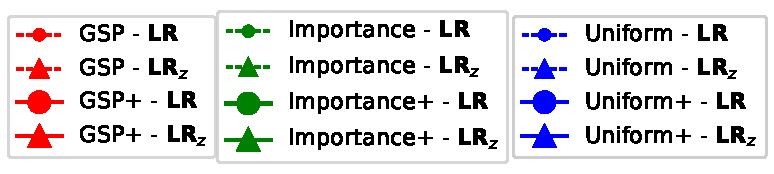
\includegraphics[width=\linewidth]{./fig/legend.pdf}
        \subcaption{图(b)、(d)的图例}
    \end{minipage}
    \\
    \begin{minipage}{0.49\linewidth}
        \centering
        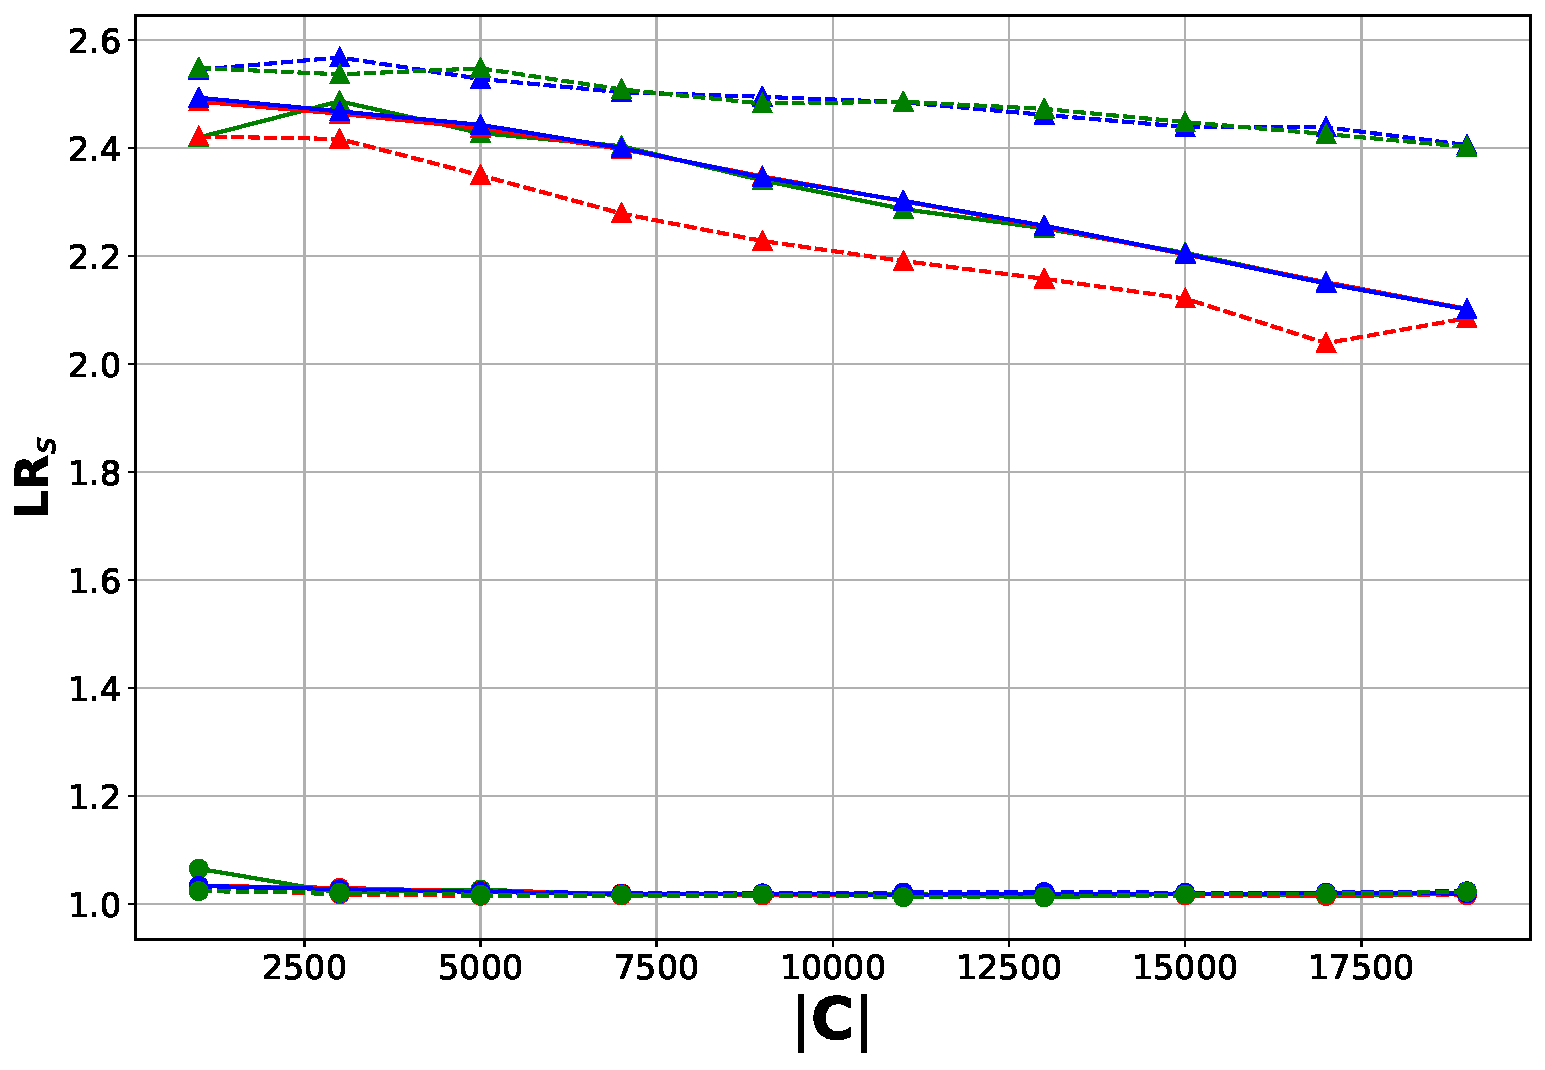
\includegraphics[width=\linewidth]{./fig/loss_ratio(0.05,0.2) - MNIST.pdf}
        \subcaption{(0.05,0.2)-MNIST $\mathbf{LR},\mathbf{LR}_z$}
    \end{minipage}
    \hfill
    \begin{minipage}{0.49\linewidth}
        \centering
        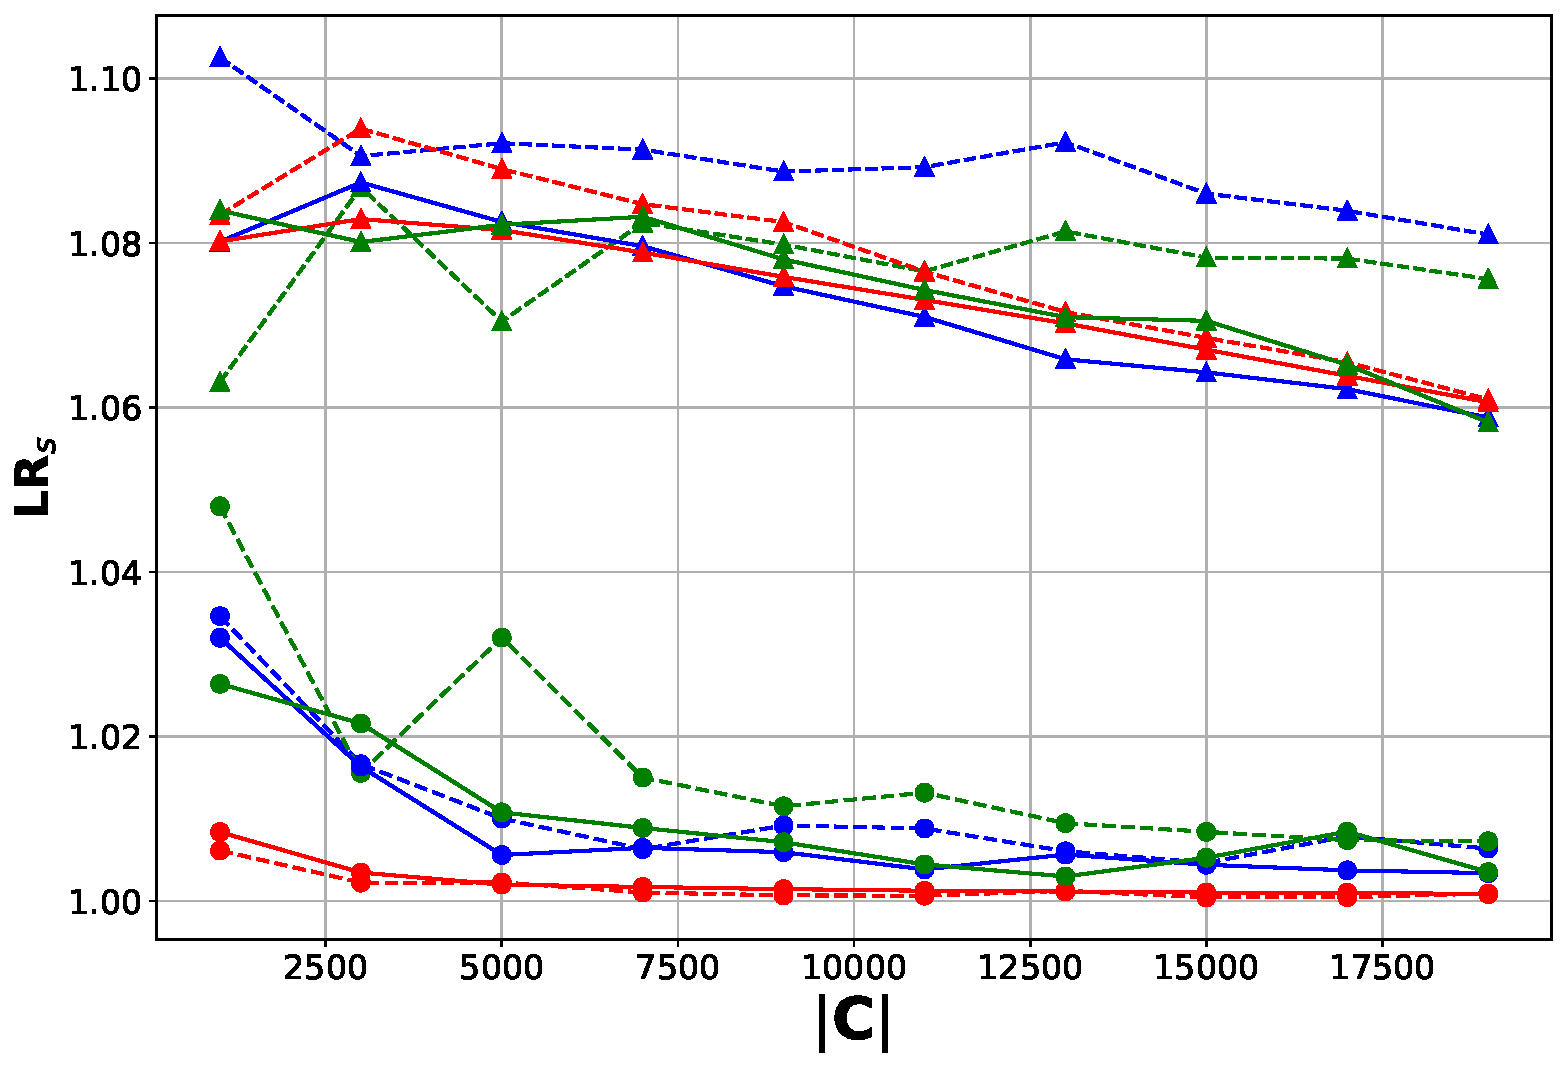
\includegraphics[width=\linewidth]{./fig/loss_ratio(0.2,0.05) - MNIST.pdf}
        \subcaption{(0.2,0.05)-MNIST $\mathbf{LR},\mathbf{LR}_z$}
    \end{minipage}
    \caption{两种参数下MNIST数据集上的表现}
    \label{fig:mnist_combined}
\end{figure}

由此可见,在实际应用过程中,如何选择合适的参数对于鲁棒算法的性能至关重要。
而本文采用的算法框架支持动态更新并重新计算核心集,其一大特点就是更新参数的效率较高。
相比于重新计算所有数据的核心集而言,本框架只需要利用“merge-and-reduce”技术就可以实现快速更新。


\begin{figure}
    \centering
    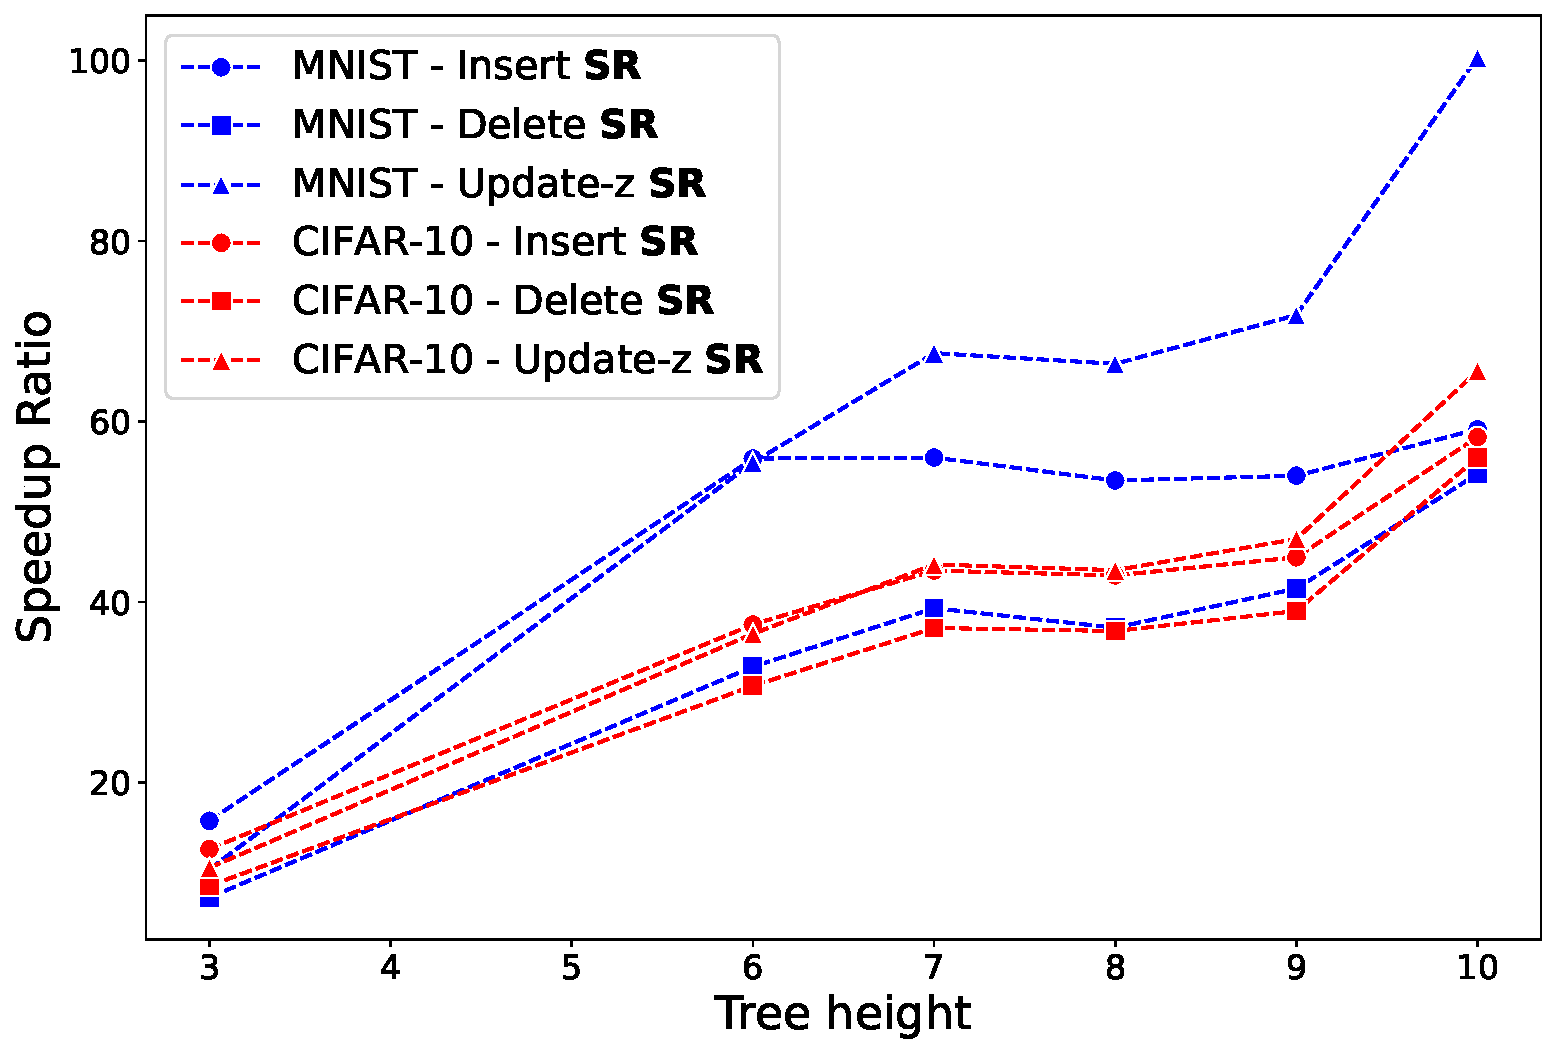
\includegraphics[width =0.6\linewidth]{./fig/dynamic.pdf}
    \caption{MNIST和CIFAR-10数据集上的动态加速比}
    \label{fig:dynamic}
\end{figure}

图\ref{fig:dynamic}是在MNIST和CIFAR-10数据集上的动态实验结果。我们选用了最为简单的均匀采样作为黑盒方法,计算在不同的树高时,其增删数据,以及变更参数
$z$的加速效果,其中Insert $\mathbf{SR}$,Delete $\mathbf{SR}$,Update-z $\mathbf{SR}$分别表示插入数据,删除数据和修改参数的加速比。

